\documentclass[10pt,twocolumn,letterpaper]{article}

\usepackage{cvpr}
\usepackage{times}
\usepackage{epsfig}
\usepackage{graphicx}
\usepackage{amsmath}
\usepackage{amssymb}

\usepackage{caption}
\usepackage{subcaption}

% Include other packages here, before hyperref.

% If you comment hyperref and then uncomment it, you should delete
% egpaper.aux before re-running latex.  (Or just hit 'q' on the first latex
% run, let it finish, and you should be clear).
%\usepackage[pagebackref=true,breaklinks=true,letterpaper=true,colorlinks,bookmarks=false]{hyperref}

\cvprfinalcopy % *** Uncomment this line for the final submission

%\def\cvprPaperID{****} % *** Enter the CVPR Paper ID here
%\def\httilde{\mbox{\tt\raisebox{-.5ex}{\symbol{126}}}}

% Pages are numbered in submission mode, and unnumbered in camera-ready
\ifcvprfinal\pagestyle{empty}\fi
\begin{document}

%%%%%%%%% TITLE
\title{Breadboard to Schematic}

\author{Catherine Olsson \\
MIT\\
{\tt\small catherio@mit.edu}
% For a paper whose authors are all at the same institution,
% omit the following lines up until the closing ``}''.
% Additional authors and addresses can be added with ``\and'',
% just like the second author.
% To save space, use either the email address or home page, not both
\and
Michele Pratusevich\\
MIT\\
{\tt\small mprat@mit.edu}
}

\maketitle
\thispagestyle{empty}

%%%%%%%%% ABSTRACT
\begin{abstract}

TODO: Write the abstract.

\end{abstract}

%%%%%%%%% BODY TEXT
\section{Introduction}

Breadboards are an important tool for do-it-yourself hardware
designers to quickly test circuit systems. They are easy to assemble,
easy to change, and easy to test, so are the tool of choice for the
first prototype of many hobbyists and students. A
programmatically-drawn, or more likely hand-drawn, schematic diagram
is used to prototype the circuit board, but if the circuit is going to
be used for high-speed, low-noise, or multiple-production
applications, a printed circuit board (PCB) is much more desirable
than a breadboard. However, it can be time-consuming to enter a
breadboard's connection map into a programmatic language that can be
used to generate a PCB. It would be faster to create a PCB-ready
representation directly from the circuitboard. Even if the result had
errors, these could be corrected by the user in less time than it
would take to create the representation from scratch.

Our approach to solve this problem was a vision-based tool to
go from a picture of a breadboard circuit to a file written in a
PCB-ready format given by Eagle. Although a fully-automated tool
proved to be too large a task for this project, we have successfully
implemented a GUI-based tool that spans the full pipeline from
bitmap image input to PCB-ready output by incorporating automated
methods with input from the user.

Overall, this project was an exercise not only in computer vision
methods for recognition and segmentation, but also in more general
problems of visualization; modularity; and designing, manipulating,
and transforming between representations on a spectrum from
concrete (pixel-level) to abstract (component-level).

%-------------------------------------------------------------------------

\section{Related Work}

TODO, if any

%-------------------------------------------------------------------------

\section{Background}

\subsection{Properties of Breadboards}

When solving vision-based problems, it is critical to know your system
properties to better develop algorithms customized to the strengths and
weaknesses of a particular application. Photos of breadboards have a number of
interesting properties that can be useful in segmentation, identification, and
restructuring tasks. A number of visually-interesting properties are listed here:
\begin{itemize}
\item A single component on a breadboard, such as a wire, LED, or chip is often a single color. 
\item The colors of the various components are often easily visually distinguishable. 
\item The breadboard is often square with the image. 
\item The breadboard, when not covered with components, has a black checkered pattern of holes in it. 
\item The breadboard color is relatively constant over the entire breadboard, except for the holes.
\item Breadboards follow a specific connectivity pattern. In Figure \ref{fig:board}, each column (not including the top two and bottom two rows) can be considered a single connection. The middle gap in the square holes is a break in the connection for each column, so there are five total holes connected to one connection in each of the columns. The top two and bottom rwo rows are connected horizontally into a single connection. Typically, one denotes a voltage of $+5$ volts and one denotes \verb|GND|, or $0$ volts. 
\end{itemize}

\begin{figure}[t]
\begin{center}
   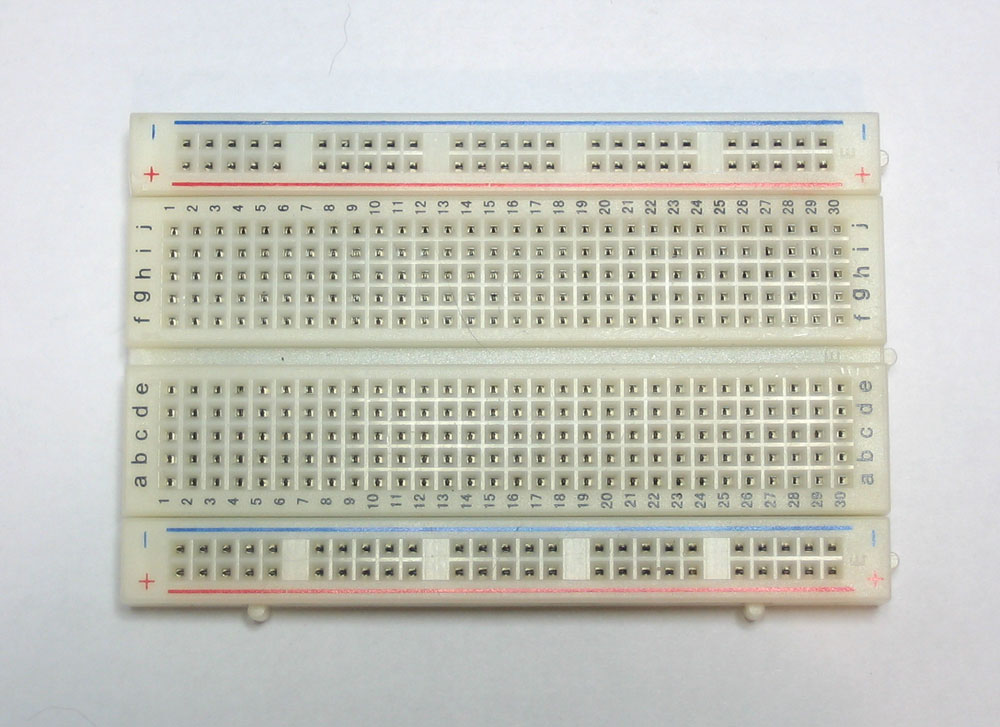
\includegraphics[width=0.8\linewidth]{imgs/breadboard.jpg}
\end{center}
   \caption{A breadboard oriented like those oriented in images that
     we can process, before any components have been added to it}
\label{fig:board}
\end{figure}

\subsection{Schematic-drawing Software}

The Eagle program, developed by CADSoft, is a free schematic and PCB-drawing
software that translates schematics into a PCB-ready format. The Eagle file
format is a type of XML, which makes it easy to programmatically update from an
image. Eagle PCB and schematic diagrams are based off of the same language, so
drawing a schematic in Eagle is sufficient to computing the full PCB. 

%-------------------------------------------------------------------------

\section{User Interface of our Tool}

From the point of view of the user, the workflow of our tool is as
follows:

\begin{enumerate}
\item Start the program, indicating the filename of the bitmap image
  containing a photograph of the breadboard.
\item Select the most important colors in the image. For example, a
  beige breadboard with red and green wires and a black microchip
  would require the user to click on examples of those four colors.
\item Confirm the selected colors to view a segmentation map of the image
  based on those colors.
\item Select the components in the segmentation map which should be
  analyzed and included in the final schematic.
\item Confirm the selected components and obtain an XML version of
  their connectivity.
\end{enumerate}

In the following sections we will explain more about our approach to
the problem, the results we obtained, and the limitations of our tool
and techniques.

%-------------------------------------------------------------------------
\section{The Approach}

The problem of translating information from a picture of a circuit to a
PCB-friendly file format has two main steps. First, the components must be
identified in the image, and second, the components must be placed in a virtual
grid representation independent of their relation in the image. 

For our implementation we chose to use python, along with the packages
Tkinter, PIL, SciPy, and Numpy, for ease of implementation, user
interface, and speed.

%-------------------------------------------------------------------------
\subsection{Segmentation into Circuit Components}

We tried two different algorithms for segmenting and detecting
components, described here. Both are color-based, and rely on the
observation that the elements of a breadboard are brightly colored, so
a rough segmentation can be found simply by grouping similarly-colored
pixels together. Of the two algorithms we tried, the second algorithm
is the one that was ultimately used in our complete system.

\subsubsection{Color Following}

As a first step to tackling the component segmentation problem, we
developed an algorithm that ``grows'' a component from a given pixel
based on its color. The basic principle is to add pixels to the set of
pixels in the component only if they do not change the average color
of the component very much. More specifically, the algorithm works as
follows: A seed pixel is given to the algorithm and added to an active
set of pixels. For each neighbor of each pixel in the active set, the
decision is made whether that pixel is in the component, if the pixel
does not change the running RGB color-average of all the pixels
current in the component. If a pixel is added to a component, it is
then also added to the active set and the algorithm continues.

The main problem with this algorithm is that it is highly dependent on the seed
pixel. The algorithm performs well when the seed pixel is close to the
average of the component it belongs to. However, if a seed pixel is
chosen which is in a given component but significantly lighter or
darker than average, the algorithm will perform poorly. Failure modes
we encountered included identifying only part of a component, or
particularly in the case of accidentally selecting too dark a pixel
near the border, determining that the shadow of a component was part
of the component and then spreading outward to include further
component shadows. 

An additional problem is that a set of seed pixels needs to be
selected first before the algorithm can grow them into components. It
is not clear how to find these seed pixels, since choosing every pixel
is too computationally expensive, but some components might get missed if only a
subset is selected.

\subsubsection{Segmentation by Nearest Color}

We implemented a second color-based segmentation algorithm which is
based on color quantization. Rather than operating locally by growing
a component from a seed pixel, this ``nearest color'' algorithm
operates over the entire image. The general idea is to quantize the
image into a small number of colors based on the colors of the
wires, chips, and other components, and then find connected components
in that color space.

More specifically, the algorithm works as follows:
\begin{enumerate}
\item \textbf{Select a palette of representative colors for
  quantization.} Ideally, a 3D clustering algorithm in RGB-space would
  be used in this step. We implemented a k-means clustering algorithm
  for use in this step, but it was too computationally intensive when
  run on the entire set of pixels to appropriate for in an interactive
  tool, and when run on a downsampled set of pixels small enough to
  run quickly, it found only shades of beige (the background
  color). In our current implementation, the user must interactively
  select colors for quantization.
\item \textbf{Map image colors to the nearest palette color.}
  In this step, each image point is mapped to the nearest color
  in the palette defined in the previous step. In effect, this step
  can be viewed as dividing up the color space into Voronoi regions
  according to Euclidean distance in RGB-space from the palette
  hues. The output of this step for a sample image is shown in Figure~\ref{fig:segment-quantized}.
\item \textbf{Find connected components of each color.} For each
  color, a connected components algorithm is run to identify
  contiguous regions of that color. The labels returned for each color
  are combined to form an overall labeling of the image into components.
\item \textbf{Eliminate small connected components using
  binary erosion/propagation.} The morphological operations of binary
  erosion and propagation are used to eliminate small regions in
  a binary image (such as our connected-components representation)
  without distorting the contours of larger objects. This feature is
  especially useful in anticipation of automatically selecting the
  components to add to the final layout according to some inclusion
  heuristic, because it cuts down on the number of
  components that must be checked by the heuristic. The output of this
  step for a sample image is shown in
  Figure~\ref{fig:segment-connected} using the pyplot ``jet'' colormap
  to visualize the labeled regions.
\end{enumerate}

This algorithm works surprisingly well on the breadboards we tested
on. However, its most obvious flaw is inability to segment
similarly-colored objects that are close together, because so much
information about shading is discarded.

One possible future direction we considered is the use of a
``watershed'' algorithm to improve the segmentation. Watershed
algorithms interpret greyscale images as relief maps and find the
``basins''. In such a relief map, the shadows on the boundaries
separating similarly-colored components would be visible, hopefully
leading to improved segmentation performance.

\begin{figure}[ht]
\centering
\begin{subfigure}[b]{\linewidth}
	\centering
   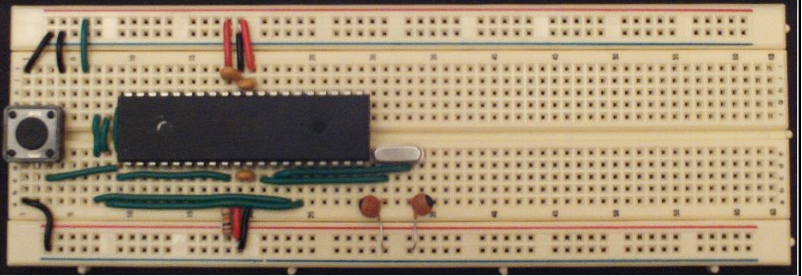
\includegraphics[width=0.9\linewidth]{demos/original_of_comp.png}
	\caption{The original image.}
	\label{fig:segment-orig}
\end{subfigure}
\begin{subfigure}[b]{\linewidth}
	\centering
   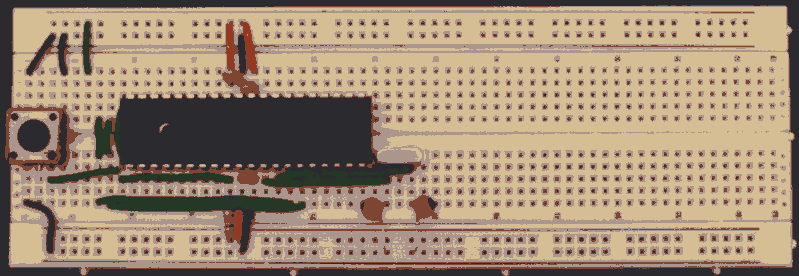
\includegraphics[width=0.9\linewidth]{demos/quantized_img2.png}
	\caption{The image after color quantization.}
	\label{fig:segment-quantized}
\end{subfigure}
\begin{subfigure}[b]{\linewidth}
	\centering
   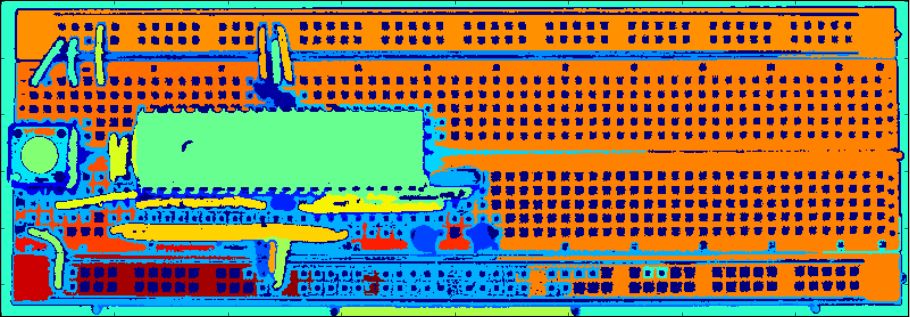
\includegraphics[width=0.9\linewidth]{demos/connectedcomponents_jet_img2.png}
	\caption{The image after identifying connected components and
      performing binary erosion and propagation. The dark blue regions
      are not identified as belonging to any component.}
	\label{fig:segment-connected}
\end{subfigure}
\end{figure}

\subsection{Virtual Grid Representation}

The next component of the project involved translating the component data into
a schematic. Knowing all the pixel locations that make up a component, we
calculate the end pixel positions of each component rounded to the nearest
$10$. Because components are aligned to the hole-grid that is present on the
breadboard, the calculated endpoints of the components can be used to place
components on a grid in the schematic. The rounded values for the $x$ and $y$
coordinates are used to place the components into their XML representations
into the schematic. 

After all components are identified and represented in their XML formats, a new
file is constructed with the proper sschematic-XML information.    

%-------------------------------------------------------------------------
\section{Results}

Running our system using the nearest-color algorithm for segmentation yielded
very positive results. Figure \ref{fig:origfull} shows the original image
operated on, and Figure \ref{fig:segfull} shows the image after
segmentation. The final schematic result (opened as a file in Eagle) is shown
in Figure \ref{fig:schemfull}. 

Notice how the schematic figure is upside down of the original image and it's
segmentation; this is a result of the difference in indexing conventions
between PIL, numpy, and Eagle.

\begin{figure}[ht]
\centering
\begin{subfigure}[b]{\linewidth}
	\centering
   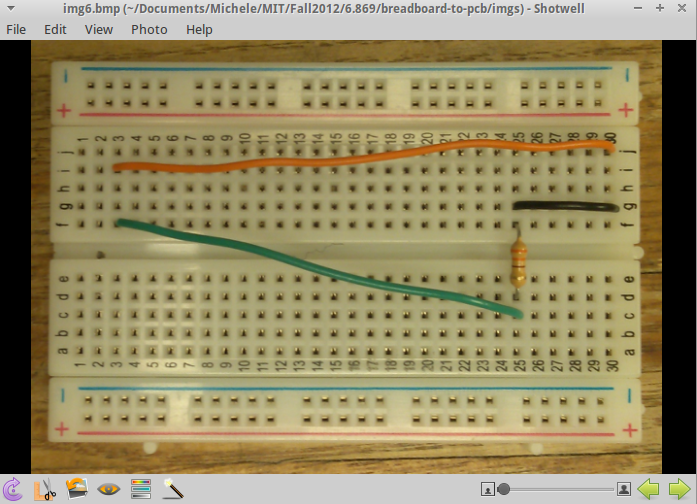
\includegraphics[width=0.9\linewidth]{demos/full_pipeline2_original.png}
	\caption{The original image}
	\label{fig:origfull}
\end{subfigure}
\begin{subfigure}[b]{\linewidth}
	\centering
   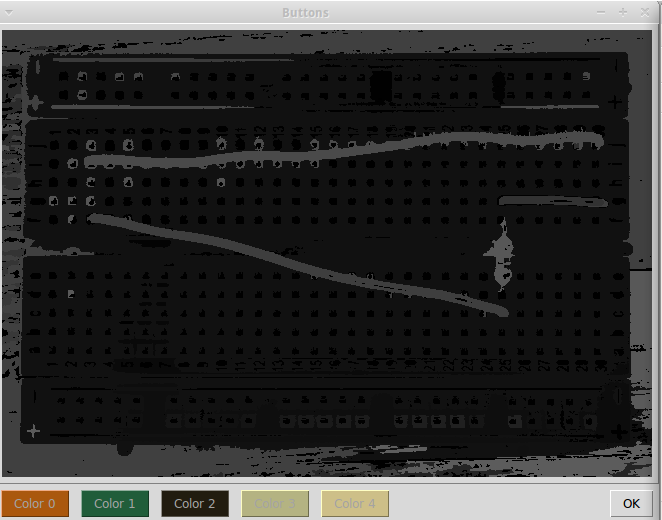
\includegraphics[width=0.9\linewidth]{demos/full_pipeline2_segmentation.png}
	\caption{The image after the segmentation into components using
      our interactive tool. This dark grey color scheme is fairly poor
    for visualization, but we could not figure out how to persuade
    Tkinter to display numeric labels using a more visible colormap
    the way pyplot is able to.}
	\label{fig:segfull}
\end{subfigure}
\begin{subfigure}[b]{\linewidth}
	\centering
   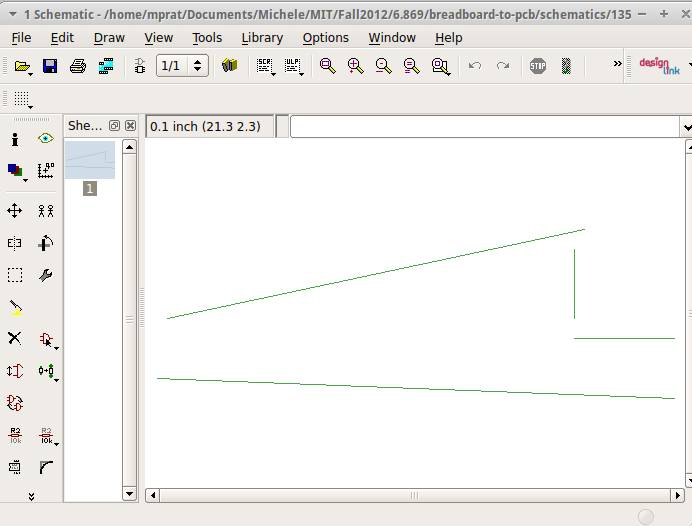
\includegraphics[width=0.9\linewidth]{demos/full_pipeline2_schematic.png}
	\caption{The schematic computed from the original image}
	\label{fig:schemfull}
\end{subfigure}
\end{figure}

\subsection{Comparing Color-following and Segmentation by Nearest Color}

The color-following and nearest-color algorithms solve somewhat different
problems. The color-following algorithm assumes a seed pixel (whether given
programmatically or by a user) and constructs a component from that seed pixel,
while the nearest-color algorithm separates the image into sections based on
colors found in the entire image. In both cases, if the same component is
found, it should be found correctly. Given that the exact parameters for both
algorithms were not perfectly tuned, these results are a comparison of the
current implementations of the algorithms as we have them.

\begin{figure}[ht]
\centering
\begin{subfigure}[b]{\linewidth}
	\centering
   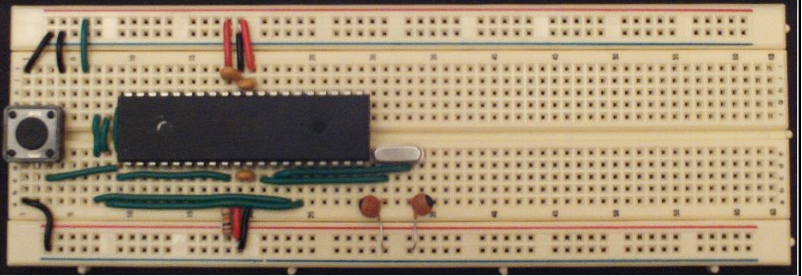
\includegraphics[width=0.9\linewidth]{demos/original_of_comp.png}
	\caption{The original image}
	\label{fig:origcomp}
\end{subfigure}
\begin{subfigure}[b]{\linewidth}
	\centering
   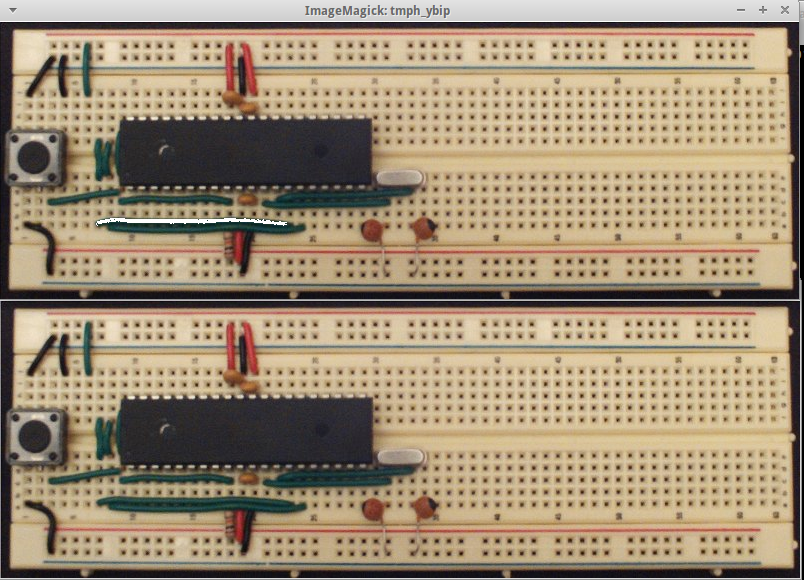
\includegraphics[width=0.9\linewidth]{demos/single_wire_not_double.png}
	\caption{The white wire detected by the color-following algorithm}
	\label{fig:cfollow}
\end{subfigure}
\begin{subfigure}[b]{\linewidth}
	\centering
   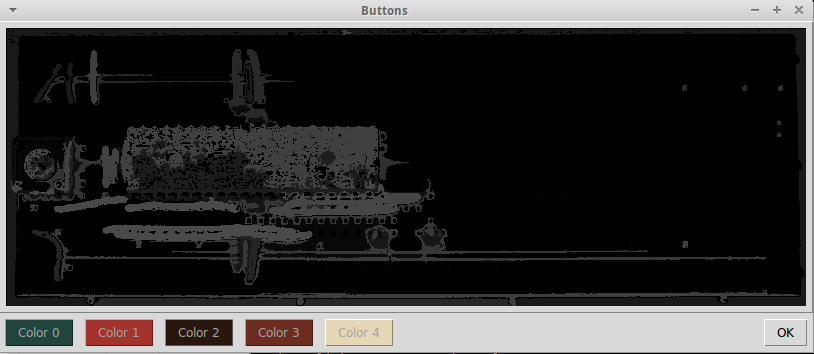
\includegraphics[width=0.9\linewidth]{demos/closest_color.png}
   \caption{Note the same wire incorrectly detected by the closet-color algorithm}
	\label{fig:ncolor}
\end{subfigure}
\end{figure}

Figure \ref{fig:origcomp} has the original image that we are analyzing. Figure
\ref{fig:cfollow} shows one wire detected by the color-following algorithm.
Note how, given a particularly good seed color, it was able to only detect one
of the two wires that are nearest each other. In Figure \ref{fig:ncolor}, note
the same wire is detected as a single wire with the wire immediately below it. 

\subsection{Limitations}

One limitation of our product as we've written it is that it can only handle
breadboard circuits that are oriented horizontally as shown above in Figure
\ref{fig:board}. This is because connectivity properties of the breadboard are
geometry-dependent, and our program automatically assumes a particular
orientation for the breadboard to infer connectivity.  

Additionally, we do not handle occlusions. A common problem with
breadboard circuits is often that components (most often wires) are
occluded from each other. This is a critical issue that in any
finalized version of a product like this needs to be
addressed.

%-------------------------------------------------------------------------
\section{Future Work}

There are several desirable features that would be useful to add to
this system:
\begin{itemize}
\item Automatically detecting components without any user
  input. Currently, the user must help the system find the initial
  colors. A more efficient color clustering algorithm would enable us
  to remove this step of user input.
\item Automatically selecting components for inclusion in the final
  schematic. Currently the user must tell the system which connected
  regions are wires or other components, and which regions should be
  ignored. Using heuristics such as size, shape, and smoothness, the
  system could determine on its own which segmented regions should be
  further processed.
  \item More sophisticated component-type identification to identify
    regions as resistors, chips, LEDs, and so on. Currently we
    identify and classify wires according to their aspect ratio /
    length, but other heuristics could be used to identify other components.
  \item More robust alignment of wires in the final schematic
    would help ensure that the schematic is physically
    correct. Currently the system aligns the wires to the nearest 10
    pixels, which has been adequate in the cases that we have tested to
    ensure that wires that should connect are mapped
    accordingly. However, there is no verification or error correction
    at this stage.
\end{itemize}

%-------------------------------------------------------------------------
\section{Conclusion}

Knowing the space of images your tool is working under greatly improves the
success of the tool you are building. It is important to know the advantages
and disadvantages of your image space when designing algorithms to achieve
vision-based goals. Transforming a circuit from the image space to the
schematic circuit space is possible with the correct parameter tuning. 

{\small
\bibliographystyle{ieee}
\bibliography{egbib}
}

\end{document}
